\documentclass[9pt,twocolumn,twoside]{../../styles/osajnl}
\usepackage{fancyvrb}
\usepackage{listings}

\journal{i524} 

\title{Big data Visualization with Apache Zeppelin}

\author[1, *]{Naveenkumar Ramaraju}
\author[1,*]{Veera Marni}

\affil[1]{School of Informatics and Computing, Bloomington, IN 47408, 
U.S.A.}


\affil[*]{Corresponding authors: naveenkumar2703@gmail.com, 
narayana1043@gmail.com}

\dates{project-008, \today}

\ociscodes{Zeppelin, Apache, Big data, Visualization}

% replace this with your url in github/gitlab
\doi{\url{https://github.com/cloudmesh/sp17-i524/blob/master/project/S17-IR-P008/report/report.pdf}}


\begin{abstract}
	Apache Zeppelin is an open source notebook for data analytics and
	visualization. In this project Apache Zeppelin is used to  deploy
	and do visual data analytics by taking advantage of parallel 
	computing capabilities of Spark in multiple cloud environments. 
	\newline
\end{abstract}

\setboolean{displaycopyright}{true}

\begin{document}
	
	\maketitle
	
	\section{Introduction}
	
	Interactive browser-based notebooks enable data engineers, data 
	analysts and Data scientists to be more productive by developing, 
	organizing, executing, and sharing data code and visualizing 
	results without referring to the command line or needing the 
	cluster details. Notebooks allow these users not only allow to 
	execute but in order to interactively work with long work-flows  
	There are a number of notebooks available with Spark. Although 
	IPython remains a mature choice and great example of a data 
	science notebooks, it has certain limitations when used for 
	visualizations with spark which are fulfilled by Apache Zeppelin. 
	
	Apache Zeppelin\cite{www-zeppelin} is a upcoming web-based 
	notebook 
	which brings data exploration, visualization, sharing and 
	collaboration features to Spark.   It supports Python and also 
	has a growing list of programming languages such as Scala, Hive, 
	SparkSQL, shell and markdown. 
	
	It is a completely open web-based notebook that enables 
	interactive data analytics used for data ingestion, discovery, 
	analytics, visualization and collaboration. It has built in Spark 
	integration and supports multiple language backends like Python, 
	Hadoop HDFS, R etc.  Multiple languages can be used within same 
	Zeppelin script and share data between them. In this project we 
	deployed Zeppelin along with in built Spark and backend 
	languages R and Python across cluster using Ansible. Then 
	installed 
	additional visualization packages provided by Apache Zeppelin 
	Helium\cite{www-helium} APIs.
	
	We also loaded a data set into Spark across cluster and 
	perform 
	data analytics and visualization in cloud using Zeppelin. However 
	since the goal of this class project is focus on deployment of 
	Big 
	data software across multiple machines and benchmarking the time 
	for 
	deployments, we focused more on that through out the 
	paper 
	and gave less importance to the analytics that are performed 
	after the deployment.
	
	\section{Infrastructure}
	
	The deployment of Apache Zeppelin is done on two clouds. The 
	clouds 
	selected for the purpose of this project are
	\begin{enumerate}
		\item Chameleon Cloud
		\item JetStream Cloud
	\end{enumerate}
	
	\subsection{OpenStack}
	
	OpenStack\cite{www-openstack} is a cloud operating system that 
	controls large pools of compute, storage, and networking 
	resources 
	throughout a data center, all managed through a dashboard that 
	gives 
	administrators control while empowering their users to provision 
	resources through a web interface. It was created as joint 
	project 
	between NASA and Rackspace that is currently managed by OpenStack 
	Foundation. It is open source software released under the Apache 
	2.0 
	license.
	
	Both Chameleon cloud and JetStream use OpenStack. OpenStack is a 
	free, open source cloud computing platform primarily deployed as 
	IaaS.\cite{www-laas}
	
	\subsection{Chameleon Cloud}
	
	Chameleon Cloud\cite{www-cc} provides a large-scale platform to 
	the 
	open research community allowing them to explore trans-formative 
	concepts in deeply programmable cloud services, design and core 
	technologies. It is funded by the National Science Foundation. 
	The 
	testbed of Chameleon Cloud is hosted at the University of Chicago 
	and 
	Texas Advanced Computing Center and the University of Chicago. 
	Chameleon provides resources to facilitate research and 
	development 
	in areas such as Infrastructure as a Service, Platform as a 
	Service, 
	and Software as a Service. Chameleon provides both an OpenStack 
	Cloud 
	and Bare Metal High-level Performance Computing 
	Resources\cite{www-bmhlpc}.
	
	\subsection{JetStream Cloud}
	
	Jetstream is led by the Indiana University Pervasive Technology 
	Institute (PTI), will add cloud-based computation to the national 
	cyberinfrastructure. Researchers will be able to create virtual 
	machines on the remote resource that look and feel like their lab 
	workstation or home machine, but are able to harness thousands of 
	times the computing power. Jetstream will provide the following 
	core 
	capabilities use Virtual Machines interactively, Researchers and 
	students can move data to and from Jetstream using {Globus 
		transfer}\cite{www-gt}, use virtual desktops and publish VMs 
		with a 
	Digital Object Identifier(DOI)\cite{www-doi}.
	
	
	
	\section{Apache Zeppelin}
	
	Apache Zeppelin is Apache project under open-source license 
	Apache 2.0. 
	It aims to provide a web interface to analyze and format large 
	volumes of data processed via spark in a visual and interactive 
	way. 
	It is a notebook style interpreter that enables collaborative 
	analysis sessions sharing between users. Zeppelin is independent 
	of 
	the execution framework itself. Current version run on top of 
	Apache 
	Spark but it has pluggable interpreter APIs to support other data 
	processing systems. More execution frameworks of type SQL-like 
	backends  such as Hive, Tajo, MRQL can also be added.
	
	\subsection{Background}
	
	Large scale data analysis workflow includes multiple steps like 
	data 
	acquisition, pre-processing, visualization, etc and may include 
	inter-operation of multiple different tools and technologies. 
	With 
	the widespread of the open source general-purpose data processing 
	systems like Spark there is a lack of open source, modern 
	user-friendly tools that combine strengths of interpreted 
	language 
	for data analysis with new in-browser visualization libraries and 
	collaborative capabilities.
	
	Zeppelin initially started as a GUI tool for diverse set of 
	SQL-over-Hadoop systems like Hive, Presto, Shark, etc. It was 
	open 
	source since its inception in Sep 2013. Later, it became clear 
	that 
	there was a need for a greater web-based tool for data scientists 
	to 
	collaborate on data exploration over the large-scale projects, 
	not 
	limited to SQL. So Zeppelin integrated full support of Apache 
	Spark 
	while adding a collaborative environment with the ability to run 
	and 
	share interpreter sessions in-browser.
	
	\subsection{Zeppelin Features}
	
	Currently, Apache Zeppelin multipurpose notebook supports the 
	following functionalities.
	\begin{enumerate}
		\item Data Ingestion
		\item Data Discovery
		\item Data Analytics
		\item Data Visualization
		\item Collaboration
	\end{enumerate}
	
	\subsection{Zeppelin Architecture}
	
	\begin{figure}
		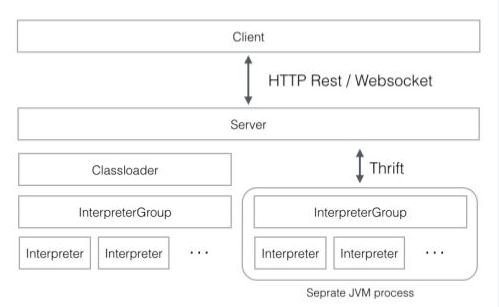
\includegraphics[width=\linewidth]{./images/zeppelin-arch}
		\caption{Zeppelin Architecture}
		\label{fig:Zeppelin Architecture}
	\end{figure}
	
	\subsubsection{Client}
	Apache Zeppelin is a client based application. Analytics can be 
	done with latest version of modern browsers. Anyone with details 
	of the host details, port on which zeppelin is listening and 
	access to the zeppelin interpreter can execute or view the 
	notebooks.
	
	\subsubsection{Server}
	Apache Zeppelin is a web-server based application. Zeppelin 
	listens on a port and application communicates to server through 
	this port. This server-client based architecture facilitates 
	sharing of notebooks and collaboration.  
	
	\subsubsection{Classloader}
	Classloader loads the essential classes and configuration for 
	running of Zeppelin. This also loads spark context as base 
	interpreter. This loads additional interpreter and their classes 
	when the new interpreters are configured and saved.
	
	\subsubsection{Multiple Language Backend}
	
	Apache Zeppelin interpreter concept allows any 
	language/data-processing-backend to be plugged into Zeppelin. 
	Currently Apache Zeppelin supports many interpreters listed below
	
	\begin{enumerate}
		\item Apache Spark
		\item Python
		\item JDBC
		\item Markdown
		\item Shell
	\end{enumerate}
	
	Adding a new language backend is simple and shown in the next 
	sections
	
	\subsubsection{Apache Zeppelin Interpreter}
	
	Apache Zeppelin interpreter is a language backend. For example to 
	use 
	python code in zeppelin, it is needed to have a python 
	interpreter. 
	Every interpreter belongs to an InterpreterGroup. Interpreters in 
	the 
	same InterpreterGroup can reference each other. For example 
	SparkSqlInterpreter can reference SparkInterpreter to get the 
	SparkContext from it while they're in the same group.
	
	InterpreterSetting is configuration of a given InterpreterGroup 
	and a 
	unit of start/stop interpreter. All interpreters in the same 
	InterpreterSetting are launched in a single, separate JVM 
	process. 
	The interpreter communicates with Zeppelin engine via Thrift.
	
	\subsubsection{Create your own Interpreter}
	
	To create a new interpreter we need extend 
	org.apache.zeppelin.interpreter class and implement some methods. 
	We 
	can also include 
	org.apache.zeppelin:zeppelin-interpreter:[version] 
	artifact in our build system and put the jars under the 
	interpreter 
	directory with a specific directory name. Zeppelin server reads 
	interpreter directories recursively and initializes interpreters 
	including the new interpreter that is recently added.
	
	There are three locations where you can store your interpreter 
	group, 
	name and other information. Zeppelin server tries to find the 
	location below. Next, Zeppelin tries to find 
	interpreter-setting.json 
	in your interpreter jar.
	
	zeppelin\_interpreter\_dir/your\_own\_interpreter\_dir/
	interpreter-settings
	
	\section{Deployment}
	
	Zeppelin works with Spark deployed across clusters. To deploy 
	Zeppelin
	and Spark across clusters, Ansible and cloudmesh client integrated
	with python CMD is used. Refer our code for implementation. Each
	component and their brief usage is explained in this section.
	
	\subsection{Cloudmesh Client}
	
	Cloudmesh client is a command line based tool to access and manage
	multiple cloud environments. Cloudmesh client can also be used to
	define security group and monitor cloud environments. Cloudmesh 
	client
	is used in the project to boot, delete and define security group 
	to
	enable firewall settings.
	
	\subsection{Ansible}
	
	Ansible is an automation tool to automate application deployment,
	maintenance and configuration management. Ansible is used to 
	deploy
	jdk, openssh, spark and zeppelin across instances that are boot 
	using
	cloudmesh client.
	
	Ansible playbook is used to write and execute automated 
	deployment. To
	deploy zeppelin and spark, playbooks are created with different 
	roles
	like zeppelin, spark, ssh, jdk, start and stop tasks for each 
	cloud with different
	variable files. Each variable file have cloud specific environment
	variables like cloud user, home folder and permissions for 
	directory
	etc. Along with the variable files and separate role files, an 
	individual playbook that calls start and stop tasks for zeppelin 
	and spark. 
	This
	is required to launch individual roles like start and stop to be
	executed through command line. 
	
	The playbook developed for deploying spark and zeppelin is 
	configured to
	install pre-built version of spark and zeppelin instead of 
	building
	from the code. Ansible downloads the prebuilt version and extract
	it. Then the extracted version is configured for cluster by 
	setting
	the IP values of master and slaves of the cluster. 
	
	Version of Zeppelin and spark is configured in a variables file to
	make it easy to customize any version of spark or zeppelin. Ports 
	on
	which zeppelin and spark listens could be configured in the same
	along with the locations in which the spark and zeppelin need to 
	be installed. 
	
	\subsection{Security - Cross SSH}
	In order for spark master and slaves to communicate, zeppelin to
	communicate with spark master cross SSH need to be enabled 
	between all
	nodes in the cluster. This is achieved by creating a SSH public 
	and
	private keys. The private key is encrypted using 'Ansible-valut' 
	and
	stored in code repository. Then at deployment time same private 
	and
	public key are distributed across cluster using ansible with
	decryption. 
	
	\subsection{Putting to gether with CMD}
	
	\subsection{Accessing applications}
	Python CMD is used to build a command line like interface to put
	cloudmesh client and ansible together. This interfaces with 
	cloudmesh
	client to boot cloud instances with required security group and
	deploy applications using ansible.
	
	Python CMD interface takes number of instances required to boot 
	and
	launches the number of instances by using cloudmesh client. Once 
	the
	instances are booted, the details of the instances are stored 
	into an
	inventory file and config files. Now using the generated 
	inventory and
	config file ansible playbook is launched. The interface has 
	options to
	set cloud and user details.
	
	This interface also has capability to deal with local network ip 
	and
	floating IP based deployment. This enables in-network deployment 
	by
	using less scarce resources without creating floating IP address. 
	To do this
	we could set master ip through interface and cloud based
	spark-zeppelin infrastructure with master-slave using only one
	floating IP.
	
	The interface also can be used to start and stop zeppelin and/or
	spark. It calls respective ansible playbooks to execute the task 
	by
	using the inventory files created earlier. 
	
	Zeppelin Notebook is accessible via latest version of browsers 
	like
	Firefox or Chrome. Zeppelin is configured to listen on port 8080 
	and
	Spark UI is available on port 8082 of master instance. By 
	launching
	the master ip and port 8080, Zeppelin is launched and Spark master
	instance can be configured in Zeppelin. Now Zeppelin is ready to 
	do
	visual analytics by taking advantage of Spark parallel computing
	capability.
	
	Spark applications can also be launched using the command line
	interface created. This invokes start-all utility of spark to 
	launch
	master and worker nodes. It is useful in the instances where spark
	need to run as application instead of using Zeppelin for only 
	analytics.
	
	\subsection{Boot and Deployment Time}
	
	The interface prints time taken to boot the instances and time 
	taken
	to deploy the application across all the nodes. The time printed 
	are
	used for benchmarking the deployment. Booting happens in sequence 
	as
	Chameleon cloud supports sequential booting operations only. Once
	booting is completed the deployment is done in parallel across
	different machines in cluster. Refer to the benchmarking section 
	for
	the time took to deployment time on different clouds.
	
	\section{Dataset Description}
	
	This is real-world dataset\cite{www-datasetdes} collected from a 
	Portuguese marketing campaign related with bank deposit 
	subscription. 
	The business goal is to find a model that can explain success of 
	a 
	contact, i.e. if the client subscribes the deposit. Such model 
	can 
	increase campaign efficiency by identifying the main 
	characteristics 
	that affect success, helping in a better management of the 
	available 
	resources (e.g. human effort, phone calls, time) and selection of 
	a 
	high quality and affordable set of potential buying customers.
	
	The increasingly vast number of marketing campaigns over time has 
	reduced its effect on the general public. Furthermore, economical 
	pressures and competition has led marketing managers to invest on 
	directed campaigns with a strict and rigorous selection of 
	contacts. 
	Such direct campaigns can be enhanced through the use of Business 
	Intelligence (BI) and Data Mining (DM) techniques.
	
	In the benchmarking section we have used three codes to benchmark 
	the Zeppelin software that we have deployed on the Chameleon and 
	Jetstream clouds. All the codes run on the same data set and 
	written in SQL. The code is explained in more detail in the 
	visualization section below
	
	\section{Benchmarking}
	
	There are 2 different approaches used in benchmarking which are 
	used 
	for the deployments on clouds where the deployment has been done. 
	They are as follows
	
	\begin{enumerate}
		\item Deployment Benchmarking
		\item Analytical Benchmarking
	\end{enumerate}
	
	{\bf \hspace{-3ex}Deployment Benchmarking}
	\\
	This benchmarking deals with the time taken for deploying Apache 
	Zeppelin across machines. Graphs are plotted to visualize the 
	time 
	taken for deployment of Apache Zeppelin with number of machines 
	on 
	x-axis and time taken on the y-axis. The command line script also 
	includes code to record the time taken for the deployment. When 
	the 
	VM's are booted inside the command line wrapper the 
	results 
	also include the amount of time taken to deploy Apache Zeppelin 
	on 
	the virtual machines. The time taken for deploying Apache 
	Zeppelin on 
	different number of machines can be recorded and plotted on a 
	graph 
	to show analyze the increase in amount of time as the number of 
	machines increases. Ideally it is excepted that the graph in the 
	curve flattens out as with increase in the number of machines.
	
	Various factors that influence the deployment benchmarking are as 
	follows.
	\begin{enumerate}
		\item The dependencies that need to be installed on all 
		machines 
		in order to deploy the software.
		\item The network traffic can effect the time taken for 
		deployment. For example a bad network might introduce delay 
		in 
		downloading the software on to the machines.
		\item The number of machines the software has to be deployed 
		on. 
	\end{enumerate}
	
	{\bf\hspace{-3ex} Analytical Benchmarking}
	\\
	This benchmarking deals with the time taking for running the 
	analytics on clouds. The same analytics are performed on all  
	clouds on which Apache Zeppelin was deployed and the performance 
	is 
	plotted on graphs
	
	Various factors that influence the analytical benchmarking are as 
	follows.
	\begin{enumerate}
		\item The size of the data set that the scientist is working 
		on. 
		As the size of the data set it take more time to download the 
		data set and split it across machines.
		\item The way the machines are configured. If all the 
		machines 
		lie on the same hardware then the network over head is 
		largely 
		reduced decreasing delays in processing.
		\item The complexity of the algorithm. A highly complex 
		algorithm 
		can take longer time time than a simpler algorithm.
		\item The size of data set can also effect the running as the 
		algorithm time complexity will increase with the size of the 
		dataset.
	\end{enumerate}
	
	Since Cloudmesh client doesn't allow parallel boot of virtual 
	machines the boot time is neglected in the deployment benchmarking
	
	\subsection{Chameleon Cloud}
	
	The Benchmarking for on Chameleon Cloud is done and explained in 
	detail the below 2 sections. The benchmarking is only performed 
	after 
	all the machines are successfully booted and ready for deployment.
	
	\subsubsection{Deployment Benchmarking}
	
	Once all the machines are boot the ansible-playbook script is 
	started 
	automatically and the time taken to deploy Apache Zeppelin on the 
	machines is clocked before the start of the deployment and after 
	the 
	end of the deployment. The difference of the end time and start 
	time 
	is the total deployment time. The graph for deployment 
	benchmarking 
	on chameleon cloud explains the various 
	times taken to deploy Apache Zeppelin across machines with 
	changes in 
	the number of machines on Chameleon Cloud.
	
	\begin{figure}
		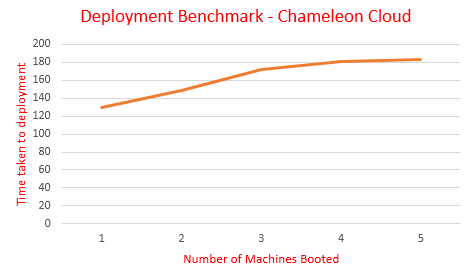
\includegraphics[width=\linewidth]{./images/chameleon_deployment_time}
		\caption{Jetstream Deployment Benchmarking}
		\label{fig:Chameleon Deployment Benchmarking}
	\end{figure}
	
	The time taken for deployment on a single machine is the lowest 
	of 
	all and the time taken for deploying more machines increases with 
	the 
	number of machines. However the graph also starts to flatten out 
	after five machines. Since the deployment is done using ansible 
	playbook the process is parallelized and all the softwares are 
	installed at the same time across all the machines. This 
	process 
	is reflected in the deployment graph shown for chameleon cloud.
	
	\subsubsection{Analytical Benchmarking}
	
	After the deployment of Apache Zeppelin on Chameleon Cloud, the 
	code 
	for the analytics is run on the Apache Zeppelin and the run time 
	is 
	clocked. The run time to process and generate the visualizations 
	is 
	plotted on the y-axis and the number of VMs in the cluster is 
	given 
	on the x-axis. The table below explains this in detail.
	
	\begin{table}[ht]
		\caption{Analytical Benchmarking Chameleon Cloud} % title of 
		%Table
		\centering % used for centering table
		Time taken to run codes Vs Machines Count \\
		\begin{tabular}{c c c c} % centered columns (4 columns)
			\hline
			\hline %inserts double horizontal lines
			VM Count & Code\#1 & Code\#2 & Code\#3 \\ [0.5ex] % 
			%inserts 
			%table
			%heading
			\hline % inserts single horizontal line
			1 & 43 & 11 & 5 \\ % inserting body of the table
			2 & 34 & 10 & 4 \\
			3 & 28 & 8 & 3 \\
			4 & 25 & 6 & 3 \\ [1ex] % [1ex] adds vertical space
			\hline %inserts single line
		\end{tabular}
		\label{table:nonlin} % is used to refer this table in the text
	\end{table}
	
	\begin{figure}
		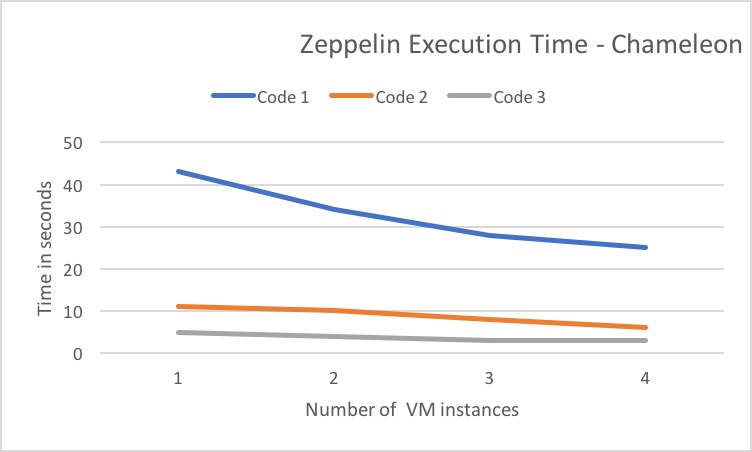
\includegraphics[width=\linewidth]{./images/Chameleon_analytic_deployment}
		\caption{Chameleon Analytics Benchmarking}
		\label{fig:Chameleon Analytics Benchmarking}
	\end{figure}
	
	\subsection{Jetstream Cloud}
	
	Similar to Chameleon Cloud, in Jetstream also cloudmesh allows 
	only 
	serial booting of VMs. Hence the boot time of the VMs is ignored 
	in 
	the process of benchmarking the deployments on the Jetstream 
	Cloud.
	
	
	\subsubsection{Deployment Benchmarking}
	
	The benchmarking in the Jetstream case is similar to that of the 
	deployment in the Chameleon cloud. The same ansible-playbook 
	script 
	is started automatically and the time taken for deployments are 
	recorded similarly. The below graph explains the amount time 
	taken to 
	deploy Apache Zeppelin on Jetsream cloud when the number of 
	machines 
	are varied.
	
	\begin{figure}
		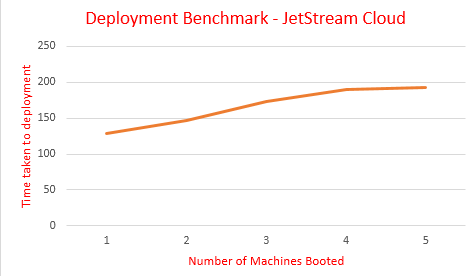
\includegraphics[width=\linewidth]{./images/jetstream_deployment_time}
		\caption{Jetstream Deployment Benchmarking}
		\label{fig:Jetstream Deployment Benchmarking}
	\end{figure}
	
	From the Jetstream deployment benchmarking figure it can be seen 
	that 
	the time taken for deploying zeppelin across virtual machines 
	stops 
	to grow and flattens out as the number of virtual machines start 
	to 
	increase. It can also be noted that there is an increase in the 
	number time taken for deployment the number of virtual machines 
	is 
	less than 4. The primary reason for this initial increase due the 
	additional overhead the master node has to handle for setting up 
	communication with the worker nodes
	
	\subsubsection{Analytical Benchmarking}
	
	Similar to the analytical benchmarking in the chameleon we also 
	performed the same experiment on Jetstream cloud. The results are 
	presented in the table below.
	
	\begin{table}[ht]
		\caption{Analytical Benchmarking Jetstream Cloud} % title of 
		%Table
		\centering % used for centering table
		Time taken to run codes Vs Machines Count \\
		\begin{tabular}{c c c c} % centered columns (4 columns)
			\hline
			\hline %inserts double horizontal lines
			VM Count & Code\#1 & Code\#2 & Code\#3 \\ [0.5ex] % 
			%inserts 
			%table
			%heading
			\hline % inserts single horizontal line
			1 & 40 & 10 & 4 \\ % inserting body of the table
			2 & 33 & 8 & 4 \\
			3 & 25 & 7 & 3 \\
			4 & 23 & 6 & 2 \\ [1ex] % [1ex] adds vertical space
			\hline %inserts single line
		\end{tabular}
		\label{table:nonlin} % is used to refer this table in the text
	\end{table}
	
	\begin{figure}
		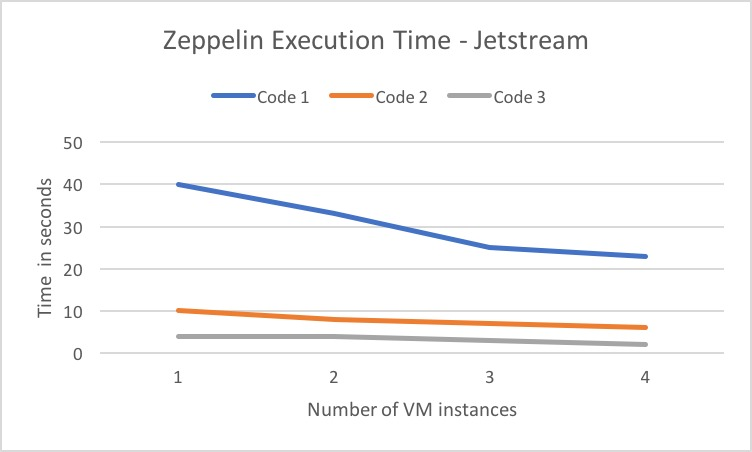
\includegraphics[width=\linewidth]{./images/Jetstream_analytic_benchmark}
		\caption{Jetstream Analytics Benchmarking}
		\label{fig:Jetstream Analytics Benchmarking}
	\end{figure}

    Analytics deployment shows a slight decrease in time as number of 
    nodes increased.
	
	\section{Visualization with Zeppelin}
	
	All the codes for visualization are written in SQL on Zeppelin. 
	Zeppelin has options to change the type of plots in a click and 
	better present the results. The basic features of zeppelin are 
	presented below through the code examples.
	
	\subsubsection{Code 1}
	
	This piece of code counts all the people who are below the age of 
	30, groups them age and then orders the counts by age. The plot 
	below shows this in detail.
	
	\begin{verbatim}
		select age, count(1) value
		from bank
		where age < 30
		group by age
		order by age
	\end{verbatim}
	
	A few of the different Types of Visualizations on the same code 
	can be seen the figures below and many others can be explored at 
	on Zeppelin basic tutorials available inbuilt in the Zeppelin 
	notebook. The figures 4, 5 and 6 show how Zeppelin plots Bar 
	Chart, Pie Chart and Line Charts on the Bank data described above.
	
	\begin{figure}
		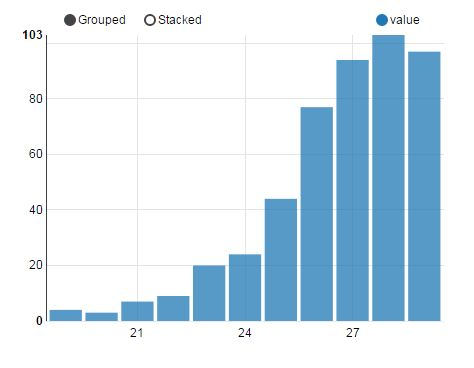
\includegraphics[width=\linewidth]{./images/code1_1}
		\caption{Histogram/ Bar Chart}
		\label{fig:Histogram}
	\end{figure}
	
	\begin{figure}
		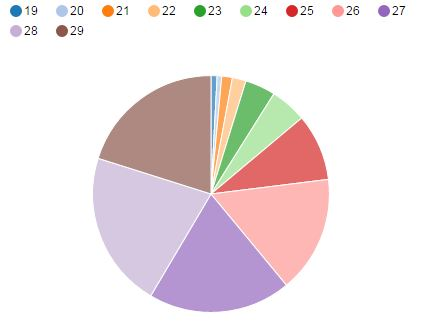
\includegraphics[width=\linewidth]{./images/code1_2}
		\caption{Pie Chart}
		\label{fig:Histogram}
	\end{figure}
	
	\begin{figure}
		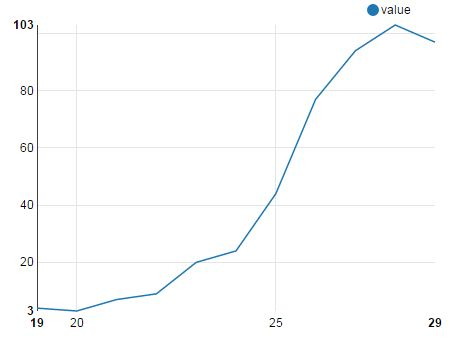
\includegraphics[width=\linewidth]{./images/code1_4}
		\caption{Line Chart}
		\label{fig:Histogram}
	\end{figure}	
	
	\subsubsection{Code 2}
	
	\begin{verbatim}
		select age, count(1) value 
		from bank 
		where age < ${maxAge=30} 
		group by age 
		order by age
	\end{verbatim}
	
	In this code above the maxAge parameter acts as an place holder 
	and excepts an user input which is an integer. After the system 
	process the user input then the place holder is replaced by the 
	input values and Zeppelin executes the code and presents the 
	results.
	
	\subsubsection{Code 3}
	
	The user input can also be a string and it shown in the code 
	below. Below code takes a string as input and processes the 
	query based on the input received 
	
	In the below query the records are picked based on the marital 
	status column, grouped by the age column and then ordered by age 
	to show the count of people on who and their age given their 
	marital status.
	
	\begin{verbatim}
		select age, count(1) value 
		from bank 
		where marital="${marital=single,single|divorced|married}" 
		group by age 
		order by age
	\end{verbatim}
	
	\section{Supplemental Material}
	
	Apache Zeppelin is Quick start tutorials are available on the 
	Apache Zeppelin webpage\cite{www-tutorial1} and can be accessed 
	for free of cost. There are also other Zeppelin works available 
	in the form of notebooks on Zeppelin hub\cite{www-zhub}.
	
	\section{Conclusion}
	
	We are successfully able to deploy Apache Zeppelin across clouds 
	with varying number of machines. The deployment time flattens out 
	after four clusters in both Chameleon and Jetstream clouds. The 
	time 
	taken to run similar zeppelin  analytic queries on both clouds 
	are 
	almost 
	similar 
	when the other parameters are fixed. 
	
	\section*{Acknowledgements}
	
	This work was done as part of the course "I524: Big Data and
	Open Source Software Projects" at Indiana University during
	Spring 2017. Thanks to our Professor Gregor von Laszewski
	and associate instructors for their help and support during the
	course.
	
	
	% Bibliography
	
	\bibliography{references}
	
	\appendix
	
	\section{Appendix}
	\subsection{Execution plan}
	
	The following subsections act as a timeline regarding how we 
	broke 
	the project up week-by-week in order to complete the entire 
	project 
	by the desired deadline. This project execution plan is a final 
	draft 
	of the project was implemented during the second half of the 
	semester.
	
	\subsubsection{March 6,2017 - March 12,201}
	
	This week we discussed about the planned how to implement the 
	project 
	in and came up with approximate deadlines for tasks. We have also 
	revisted the tutorials on the class webpage and referred to 
	official 
	documentation of Apache Zeppelin and came up with a workflow for 
	implementing this project.
	
	\subsubsection{March 13,2017 - March 18,201}
	
	This week we have installed Cloudmesh on our local machines, 
	completed the tutorials on Cloudmesh present on the class 
	website. We 
	have also accessed on chameleon cloud accounts to boot Vitrual 
	Machines on cloud and logged in successfully into the Virtual 
	Machines.
	
	We have discussed about building a command shell through which 
	we can deploy the clusters with less effort. Hence we looked 
	completed the tutorials on CMD and CMD5 available on the class 
	website. This tutorials have helped us in coming up with a basic 
	outline of the shell that we should develop in order to meet the 
	requirements for deploying Apache Zeppelin on various clouds. We 
	have 
	made a decision to use CMD module in python for this purpose.
	
	\subsubsection{March 19,2017 - March 26,201}
	
	During this week we have completed the development of the command 
	shell which can start a given number of virtual machines are 
	return 
	their details like the machine name, floating IPs, Static IPs to 
	a 
	file. Other methods like delete, setCloud, getStaticIps, 
	getFloatingIps are also included in the command shell developed 
	over 
	the week.  The description for all methods is documented and can 
	accessed from with the shell.
	
	We have discussed the over the deployment of Apache Zeppelin and 
	came 
	up with the dependencies that need to installed on the machines 
	before zeppelin in deployed on to them. We have revisted the 
	ansible 
	tutorials on the class website as we will using ansible to deploy 
	Apache Zeppelin on various clouds
	
	\subsubsection{March 27,2017 - April 2,201}
	
	Developed and tested code to deploy the Apache Zeppelin on the 
	clusters. Upon successful deployment we have opened ports so that 
	Apache Zeppelin can be accessed through web-interfaces.
	
	\subsubsection{April 10,2017 - April 16,201}
	
	Integrated the deployment code into the command shell developed 
	previously and tested the deployment chameleon cloud. We have ran 
	into issues with security and VM accessibility. We have fixed the 
	below issues over the week.
	\begin{enumerate}
		\item Fixed deployment issues that might arise to lack of 
		availability of  floating point IPs on the chameleon cloud. 
		\item Fixed security issues and checked if the notebook is 
		accessible through the external web-browsers.
	\end{enumerate}
	
	During the week we have also worked on analytics which can be 
	performed on the Apache Zeppelin that has been previously 
	installed 
	on the cloud from a web-page on in external machine. More details 
	about the analytics are discussed in the analytics section below.
	
	\subsubsection{April 17,2017 - April 23,201}
	
	Review of deployment and developing the final draft of the report 
	for 
	submission.
	
	\section*{Author Biographies}
	\begingroup
	\setlength\intextsep{0pt}
	\begin{minipage}[t][3.2cm][t]{1.0\columnwidth} % Adjust height 
		%[3.2cm] as required for separation of bio photos.
		\begin{wrapfigure}{L}{0.25\columnwidth}
			
\includegraphics[width=0.25\columnwidth]{images/john_smith.eps}
		\end{wrapfigure}
		\noindent
		{\bfseries Naveenkumar Ramaraju} yet to update his 
		Bio\end{minipage}
	\begin{minipage}[t][3.2cm][t]{1.0\columnwidth} % Adjust height 
		%[3.2cm] as required for separation of bio photos.
		\begin{wrapfigure}{L}{0.25\columnwidth}
			
\includegraphics[width=0.25\columnwidth]{images/alice_smith.eps}
		\end{wrapfigure}
		\noindent
		{\bfseries Veera Marni} yet to update his bio
	\end{minipage}
	
	\endgroup
	
	\newpage
	
\end{document}
